% Options for packages loaded elsewhere
% Options for packages loaded elsewhere
\PassOptionsToPackage{unicode}{hyperref}
\PassOptionsToPackage{hyphens}{url}
\PassOptionsToPackage{dvipsnames,svgnames,x11names}{xcolor}
%
\documentclass[
  ngerman,
  titlepage=true,
  listof=totoc]{scrartcl}
\usepackage{xcolor}
\usepackage[top=30mm,bottom=30mm,left=25mm,right=25mm]{geometry}
\usepackage{amsmath,amssymb}
\setcounter{secnumdepth}{-\maxdimen} % remove section numbering
\usepackage{iftex}
\ifPDFTeX
  \usepackage[T1]{fontenc}
  \usepackage[utf8]{inputenc}
  \usepackage{textcomp} % provide euro and other symbols
\else % if luatex or xetex
  \usepackage{unicode-math} % this also loads fontspec
  \defaultfontfeatures{Scale=MatchLowercase}
  \defaultfontfeatures[\rmfamily]{Ligatures=TeX,Scale=1}
\fi
\usepackage{lmodern}
\ifPDFTeX\else
  % xetex/luatex font selection
\fi
% Use upquote if available, for straight quotes in verbatim environments
\IfFileExists{upquote.sty}{\usepackage{upquote}}{}
\IfFileExists{microtype.sty}{% use microtype if available
  \usepackage[]{microtype}
  \UseMicrotypeSet[protrusion]{basicmath} % disable protrusion for tt fonts
}{}
\makeatletter
\@ifundefined{KOMAClassName}{% if non-KOMA class
  \IfFileExists{parskip.sty}{%
    \usepackage{parskip}
  }{% else
    \setlength{\parindent}{0pt}
    \setlength{\parskip}{6pt plus 2pt minus 1pt}}
}{% if KOMA class
  \KOMAoptions{parskip=half}}
\makeatother
% Make \paragraph and \subparagraph free-standing
\makeatletter
\ifx\paragraph\undefined\else
  \let\oldparagraph\paragraph
  \renewcommand{\paragraph}{
    \@ifstar
      \xxxParagraphStar
      \xxxParagraphNoStar
  }
  \newcommand{\xxxParagraphStar}[1]{\oldparagraph*{#1}\mbox{}}
  \newcommand{\xxxParagraphNoStar}[1]{\oldparagraph{#1}\mbox{}}
\fi
\ifx\subparagraph\undefined\else
  \let\oldsubparagraph\subparagraph
  \renewcommand{\subparagraph}{
    \@ifstar
      \xxxSubParagraphStar
      \xxxSubParagraphNoStar
  }
  \newcommand{\xxxSubParagraphStar}[1]{\oldsubparagraph*{#1}\mbox{}}
  \newcommand{\xxxSubParagraphNoStar}[1]{\oldsubparagraph{#1}\mbox{}}
\fi
\makeatother


\usepackage{longtable,booktabs,array}
\newcounter{none} % for unnumbered tables
\usepackage{calc} % for calculating minipage widths
% Correct order of tables after \paragraph or \subparagraph
\usepackage{etoolbox}
\makeatletter
\patchcmd\longtable{\par}{\if@noskipsec\mbox{}\fi\par}{}{}
\makeatother
% Allow footnotes in longtable head/foot
\IfFileExists{footnotehyper.sty}{\usepackage{footnotehyper}}{\usepackage{footnote}}
\makesavenoteenv{longtable}
\usepackage{graphicx}
\makeatletter
\newsavebox\pandoc@box
\newcommand*\pandocbounded[1]{% scales image to fit in text height/width
  \sbox\pandoc@box{#1}%
  \Gscale@div\@tempa{\textheight}{\dimexpr\ht\pandoc@box+\dp\pandoc@box\relax}%
  \Gscale@div\@tempb{\linewidth}{\wd\pandoc@box}%
  \ifdim\@tempb\p@<\@tempa\p@\let\@tempa\@tempb\fi% select the smaller of both
  \ifdim\@tempa\p@<\p@\scalebox{\@tempa}{\usebox\pandoc@box}%
  \else\usebox{\pandoc@box}%
  \fi%
}
% Set default figure placement to htbp
\def\fps@figure{htbp}
\makeatother



\ifLuaTeX
\usepackage[bidi=basic,shorthands=off]{babel}
\else
\usepackage[bidi=default,shorthands=off]{babel}
\fi
\ifLuaTeX
  \usepackage{selnolig} % disable illegal ligatures
\fi


\setlength{\emergencystretch}{3em} % prevent overfull lines

\providecommand{\tightlist}{%
  \setlength{\itemsep}{0pt}\setlength{\parskip}{0pt}}



 


\AtBeginDocument{
\hypersetup{
  colorlinks=true,
  citecolor=black
  }
}
\usepackage{XCharter}
\usepackage{float}
\usepackage{listings}
\usepackage{booktabs}
\usepackage{scrlayer-scrpage}
\pagestyle{scrheadings}
\clearpairofpagestyles
\KOMAoptions{headsepline=0.5pt}
\graphicspath{{./}{init/}}
\chead{\fontsize{14}{12}\selectfont{Abschlussbericht Praxissemester}}
\ihead{\includegraphics[scale=0.3]{Logo_klein.pdf}}
\ohead{\includegraphics[scale=0.01]{Airbus.png}}
\cfoot{\pagemark}
\makeatletter
\@ifpackageloaded{caption}{}{\usepackage{caption}}
\AtBeginDocument{%
\ifdefined\contentsname
  \renewcommand*\contentsname{Inhaltsverzeichnis}
\else
  \newcommand\contentsname{Inhaltsverzeichnis}
\fi
\ifdefined\listfigurename
  \renewcommand*\listfigurename{Abbildungsverzeichnis}
\else
  \newcommand\listfigurename{Abbildungsverzeichnis}
\fi
\ifdefined\listtablename
  \renewcommand*\listtablename{Tabellenverzeichnis}
\else
  \newcommand\listtablename{Tabellenverzeichnis}
\fi
\ifdefined\figurename
  \renewcommand*\figurename{Abbildung}
\else
  \newcommand\figurename{Abbildung}
\fi
\ifdefined\tablename
  \renewcommand*\tablename{Tabelle}
\else
  \newcommand\tablename{Tabelle}
\fi
}
\newcommand*\listoflistings\lstlistoflistings
\AtBeginDocument{%
\renewcommand*\lstlistlistingname{Listingverzeichnis}
}
\makeatother
\makeatletter
\makeatother
\makeatletter
\@ifpackageloaded{caption}{}{\usepackage{caption}}
\@ifpackageloaded{subcaption}{}{\usepackage{subcaption}}
\makeatother
\usepackage{bookmark}
\IfFileExists{xurl.sty}{\usepackage{xurl}}{} % add URL line breaks if available
\urlstyle{same}
\hypersetup{
  pdftitle={Erste Ansteuerungen},
  pdflang={de},
  colorlinks=true,
  linkcolor={black},
  filecolor={Maroon},
  citecolor={Blue},
  urlcolor={Blue},
  pdfcreator={LaTeX via pandoc}}


\title{Erste Ansteuerungen}
\author{}
\date{}
\begin{document}
\begin{titlepage}
    \noindent
    \begin{minipage}[c]{0.45\textwidth}
        \centering
        \includegraphics[scale=0.15]{Logo_groß.pdf}
    \end{minipage}
    \hfill 
    \begin{minipage}[c]{0.45\textwidth}
        \centering
        \includegraphics[scale=0.055]{Airbus.png}
    \end{minipage}

    \vspace{1.2cm}
    
    \begin{center}
        {\huge\bfseries Abschlussbericht Praxissemester \par}
        \vspace{4mm}
        {\LARGE Machbarkeitsstudie zur Weiterentwicklung eines Industrie-3D-Druckers \par}
    \end{center}
    
    \vspace{1.5cm}
    
    \begin{center}
        \large
        \begin{tabular*}{\textwidth}{@{\extracolsep{\fill}}p{7.5cm}l} 
        \toprule
        Student & Mirco Ick \\
        Matrikelnummer & 5312533 \\[1em]
        
        Datum der Abgabe & 04.11.2026 \\
        Praktikums-Zeitraum & 03.08.2026 - 04.11.2026 \\[1em]
        
        Mentor & Prof. Dr.-Ing. Mirco Meiners \\
        & mirco.meiners@hs-bremen.de \\
        Lehranstalt & Hochschule Bremen \\
        & Neustadtswall 30 \\
        & 28199 Bremen \\[1em]
        
        Betrieblicher Betreuer & M. Sc. Ken Matsubara \\
        & ken.matsubara@airbusds-airborne.com \\
        & +49 421 844881710 \\[1em]
        
        Unternehmen & Airbus DS Airborne Solutions GmbH \\
        & Richard-Dunkel-Straße 121 \\
        & 28199 Bremen \\
        \bottomrule
        \end{tabular*}
    \end{center}
\end{titlepage}
\clearpage

\tableofcontents
\clearpage
\listoffigures
\listoftables

Nachdem nun die Grundlagen des 3D-Drucks recherchiert und verstanden
wurden, konnte an die Bauteilanalyse sowie Ansteuerung erster
entscheidender Komponenten mittels Python gemacht werden. Im ersten
Schritt wurde sich hierbei um die Grundkomponenten eines 3D-Druckers
beschäftigt. Die nachfolgenden Unterkapitel werden näher auf die
Vorgehensweise und die daraus entstehenden Erkenntnisse eingehen. Alle
erwähnten Skripte sowie Datenblätter und ergänzende Dokumentationen sind
dem Github-Repository {[}@Github{]} zu entnehmen.

\subsection{Grundkomponenten eines
3D-Druckers}\label{grundkomponenten-eines-3d-druckers}

Um einen 3D-Drucker betreiben zu können braucht es prinzipiell drei
verschiedene Baugruppen. Diese drei existenziellen Baugruppen sind:

\begin{itemize}
\tightlist
\item
  Step-Motoren (Schrittmotoren): Steuern die horizontale sowie vertikale
  Bewegung des Druckkopfes über die X-/Y-/Z-Achse sowie die Steuerung
  des Filamentausschubs über den Extruder.
\item
  Endschalter: Kommunikation mit den Step-Motoren ob ein Ende der Achsen
  erreicht wurde, um die Bewegung zu stoppen sowie die Position zu
  kalibrieren.
\item
  Heizkomponenten: Erwärmung des Filaments im Hotend (Druckkopf) sowie
  bei Bedarf des Heatbeds (Heizbett).
\end{itemize}

\subsubsection{Step-Motoren}\label{sec-step}

So gut wie alle in modernen 3D-Druckern verbauten Schrittmotoren
funktionieren identisch. Es gibt vier Adern, welche an vier verschiedene
im Motor sitzende Kontakte geführt werden. Diese Kontakte sind mit zwei
voneinander getrennten Spulen verbunden, welche bei Stromfluss ein
Magnetfeld erzeugen. Dieses Magnetfeld sorgt dafür, dass sich der Rotor
des Motors in eine bestimmte Position dreht. Somit lässt sich der Motor
sehr präzise und gezielt über das erzeugte Magnetfeld kontrollieren.
Sind die Positionen bzw. Winkel in Korrelation mit den Kontakten
bekannt, kann mit dem Motor eine Rotationsbewegung durchgeführt werden.
Die Nachfolgende Abbildung~\ref{fig-step_wiring} zeigt den internen
Aufbau dieser Step-Motoren in Verbindung mit den Steuerkontakten, oft
als A+/A-/B+/B-, A1/A2/B1/B2 oder A/B/C/D bezeichnet. Neben der
Schaltung ist in der Abbildung~\ref{fig-step_sequence} die standard
Reihenfolge der Ansteuerung dargestellt.

\begin{figure}

\begin{minipage}[t]{0.50\linewidth}

\centering{

\includegraphics[width=0.5\linewidth,height=\textheight,keepaspectratio]{pics/step.png}

}

\subcaption{\label{fig-step_wiring}}

\end{minipage}%
%
\begin{minipage}[t]{0.50\linewidth}

\centering{

\pandocbounded{\includegraphics[keepaspectratio]{pics/sequence.png}}

}

\subcaption{\label{fig-step_sequence}}

\end{minipage}%

\caption{\label{fig-step_motor}Step-Motor Aufbau {[}@step\_motor{]}}

\end{figure}%

Anhand dieser Erkenntnisse wurde versucht diese Motoren anzusteuern. Da
jedoch ein Raspberry Pi nicht direkt den Strom bei der benötigten
Spannung bereitstellen kann, muss ein Motortreiber zwischengeschaltet
werden. Für diesen Versuch wurde ein bereits vorhandener \emph{L298N
Dual H-Bridge Motor Driver} verwendet. Dieser Treiber hat passend zu den
vier Kontakten des Motors ebenfalls vier Anschlüsse, welche ein
Steuersignal vom Raspberry Pi 5 entgegennehmen um den Motor anzusteuern.
Somit konnte der Motor über die GPIO-Pins des Raspberry Pi 5 angesteuert
werden. Es wurde ein kleines Skript in Python
(\texttt{4\_wire\_step.py}) geschrieben, welches die Ansteuerung der
Kontakte in der in Abbildung~\ref{fig-step_sequence} zu sehende
Reihenfolge ansteuert. Um eine volle Funktion zu erzielen fehlte noch
die Drehrichtungsänderung sowie die Einbindung der \emph{Steps}
(Motorschritte) und die Geschwindigkeitsänderung zur präzisen Steuerung.
Die Drehrichtungsänderung konnte durch die Invertierung der
Ansteuerungsreihenfolge der Kontakte umgesetzt werden. Die Einbindung
der Motorschritte wurde über einen Counter im Code umgesetzt. Dieser
zählt die Anzahl der Ansteuerungen und unterbricht die Schleife bei
Erreichen der gewünschten Zahl. Somit kann der Motor gezielt um eine
bestimmte Anzahl an \emph{Steps} gedreht werden. Die
Geschwindigkeitsänderung des Motors kann über die Zeitabstände zwischen
den verschiedenen Ansteuerungen der Kontakte geregelt werden. Jedoch sei
angemerkt, dass bei höherer Drehzahl proportional das Drehmoment sinkt.
Bei zu wenig Drehmoment kann der Motor die benötigte Anfangsleistung
nicht mehr aufbringen und es kommt zu keiner Bewegung.

\subsubsection{Endschalter}\label{sec-limit_switch}

Ein Endschalter ist nichts Weiteres als ein handelsüblicher Taster,
welcher bei Kontakt einen \emph{Normally Closed} Kontakt öffnet oder
einen \emph{Normally Opend} Kontakt schließt. Es gibt bei physischen
Endschaltern meist drei Adern, welche einen gemeinsamen Spannungs- bzw.
Ground-Kontakt, ein NO-Kontakt und einen NC-Kontakt beinhalten. Wird nun
der Schalter gedrückt wird die angeschlossene Spannung bzw. der
angeschlossene Ground weitergegeben oder unterbrochen, was eine
Zustandsänderung für das ausgehende Signal bedeutet. Diese
Zustandsänderung lässt sich nun in Bezug auf z.B. die Motoren setzen.

Hierfür wurde nun ein kleines einzelnes Python-Skript
(\texttt{limit\_switch.py}) geschrieben, welches die Funktion des
Endschalters testet und validiert. Anschließend wurde in die Funktion
der Step-Motoren ein Endschalter mit eingebaut, womit der Motor bei
Bedarf gestoppt werden kann.

\subsubsection{Heizkomponenten}\label{sec-pwm}

Die Heizelemente sind wohl die am einfachsten anzusteuerden Bauteile in
dieser Liste, da sie bei einer anliegenden Spannung Wärme erzeugen. Die
hier in einem Material eingebaute Spule, z.B. in das Hotend oder Heatbed
des Druckers, erwärmt sich bei Stromdurchfluss. Neben den Heizelementen
bedarf es jedoch noch mindestens eines Temperatursensors, welcher die
Temperatur überwacht und als Heizstopp fungiert. Diese
Temperatursensoren können als NTC (Heißleiter) oder PTC (Kaltleiter)
umgesetzt werden. Am beliebtesten sind hier jedoch die wie ein PTC
funktionierenden Platin-Sensoren, da diese PT100 bzw. PT1000 Glieder
einen sehr linearen Kurvenverlauf aufweisen. Außerdem sind sie so
optimiert, dass sie bei einer Temperatur von \(T=0\,°C\) exakt einen
Widerstand von \(R_{PT100}=100\,\Omega\) bzw.
\(R_{PT1000}=1000\,\Omega\) aufweisen. Sie sind somit ausgezeichnet für
die Temperaturmessung geeignet. Die Abbildung~\ref{fig-pt100_pt1000}
zeigt einen Kurvenverlauf der beiden Temperatursensoren.

\newpage

\begin{figure}

\centering{

\pandocbounded{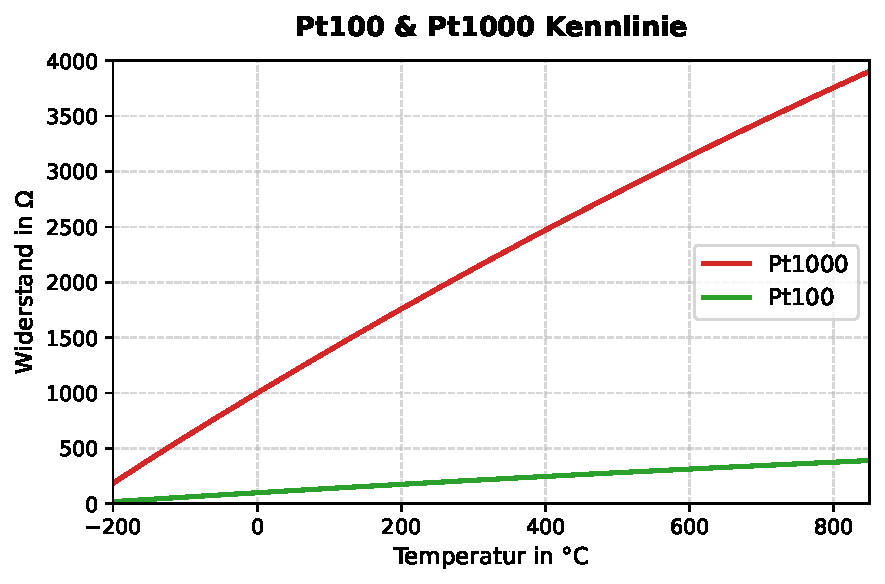
\includegraphics[keepaspectratio]{4_first_steps_files/figure-pdf/fig-pt100_pt1000-output-1.pdf}}

}

\caption{\label{fig-pt100_pt1000}Kennlinie der Pt100 und Pt1000
Sensoren}

\end{figure}%

Neben den Temperatursensoren sind außerdem noch Lüfter von Vorteil um
das Bauteil wieder abzukühlen bzw. die benötigte Temperatur zu halten
und nicht zu überschreiten. Standardisierte Lüfter beim 3D-Druck können
mit bis zu 24V über ein PWM-Signal betrieben werden. So wird über die
Pulsbreite der Signale die Spannung festgelegt. Als Beispiel kann man
einen \(5\,\text{V}\) Lüfter in Verbindung mit einer maximalen
Signalspannung von \(V_{sig}=5\,\text{V}\) nehmen. Dieses
kontinuierliche \(5\,\text{V}\) Spannungssignal entspricht für den
Lüfter eine Leistung am Ausgang von \(P_{max}=100\,\%\). Wird nun
mithilfe der Pulsweitenmodulation das Signal auf \(50\,\%\) reduziert,
das heißt es wird kein Dauerimpuls gesendet, sondern ein Impuls mit
einer Pulsbreite von \(t_{an}=50\,\%\) gesendet, so wird die Spannung
auf \(V_{sig}=2,5\,\text{V}\) reduziert und der Lüfter läuft nur noch
mit \(P=50\,\%\). Somit kann die Leistung des Lüfters über das
PWM-Signal geregelt werden. Die Abbildung~\ref{fig-pwm} zeigt die
entstehende Signalspannung bei beispielhaften PWM-Signalen.

\begin{figure}

\centering{

\pandocbounded{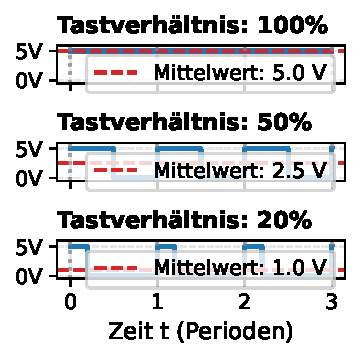
\includegraphics[keepaspectratio]{4_first_steps_files/figure-pdf/fig-pwm-output-1.pdf}}

}

\caption{\label{fig-pwm}Signalverlauf bei Pulsweitenmodulation}

\end{figure}%

\newpage

\subsection{Referenzsystem: Geeetech
i3}\label{referenzsystem-geeetech-i3}

Nach Ansteuerung der einzelnen Basiskomponenten wurde probiert mittels
eines Referenzdruckers die Bauteile anzusteuern. Dazu wurde ein
ausgesonderter \emph{Geeetech i3} 3D-Drucker verwendet, welcher
hardwareseitig über einen \emph{Arduino Mega 2560} betrieben wird. Die
Abbildung~\ref{fig-i3} zeigt das verwendete Referenzsystem.

\begin{figure}

\begin{minipage}[t]{0.50\linewidth}

\begin{figure}[H]

\centering{

\includegraphics[width=0.65\linewidth,height=\textheight,keepaspectratio]{pics/IMG_2011.jpg}

}

\caption{\label{fig-i3}Geeetech i3 Referenzsystem}

\end{figure}%

\end{minipage}%
%
\begin{minipage}[t]{0.50\linewidth}

\begin{figure}[H]

\centering{

\includegraphics[width=1\linewidth,height=\textheight,keepaspectratio]{pics/i3_aufbau.jpeg}

}

\caption{\label{fig-final_i3}Finaler Aufbau des Referenzsystems}

\end{figure}%

\end{minipage}%

\end{figure}%

\subsubsection{Festlegung der Software}\label{festlegung-der-software}

Da bereits der Arduino sowie der Raspberry Pi 5 zur Verfügung standen,
wurde sich nun auf die Lösung der Ansteuerung mittels zwei Boards
entschieden. Somit sollte der Arduino als Hardwaresteuerung und der
Raspberry Pi 5 für die komplexere Softwaresteuerung verantwortlich sein.
Für diese Art von Ansteuerung gibt es bereits sämtliche Open-Source
Lösungen. Unter anderem \emph{Klipper}, \emph{Marlin}, \emph{RRF} oder
auch \emph{Kalico}. Nach Recherchen hat sicher ergeben, dass die wohl
meist verbreitete und zugänglichste Variante \emph{Klipper} ist. Klipper
bietet mit der in Python programmierten Funktionsklassen leichte
Anpassungs- sowie Erweiterungsmöglichkeiten und für sehr viele Lösungen
bereits vorgefertigte bauteilspezifische Module. Außerdem kann mit Hilfe
von \emph{Mainsail} und \emph{Moonraker} leicht eine IP adressenbasierte
Benutzeroberfläche für Klipper geschaffen werden, mit welcher sich alle
Komponenten steuern lassen und Änderungen im Code vorgenommen werden
können. Neben dieser Weboberfläche kann zusätzlich mit \emph{Crowsnest}
eine Kamera eingebunden und mit \emph{Klipper-Screen} diese
Weboberfläche auch auf dem am Raspberry Pi angeschlossenen Display
angezeigt werden. Zusätzlich können über G-Code direkt in der
Weboberfläche Makros erstellt werden, welche die Ansteuerung der
einzelnen Komponenten vereinfachen oder z.B. eine Startsequenz für den
Drucker erstellt. Alle benötigten Softwares sind einfach über deren
eigenen Github-Repositories, direkt aus der Konsole des Raspberry Pis,
zu installieren und zu konfigurieren. Aus diesem Grund bietet Klipper
alles für die erfolgreiche Umsetzung des Projektes und wird als Software
verwendet.

\newpage

\subsubsection{Ansteuerung des
Referenzsystems}\label{ansteuerung-des-referenzsystems}

Die Ansteuerung des Referenzsystems gestaltete sich mithilfe von Klipper
und den bereits vorhandenen Modulen sowie der vorherigen Recherche der
einzelnen Komponenten einfach und nachvollziehbar. Als MCU für das
Referenzsystem wurde ein \emph{Arduino Mega 2560} mit einem \emph{RAMPS
1.4} Board verwendet, welches bereits die benötigten Anschlüsse für die
Step-Motoren, Endschalter und Heizkomponenten bereitstellt. Um nun eine
Verbindung zwischen dem Raspberry Pi 5 und dem Arduino herzustellen
musste der Arduino zuerst mit der Klipper-Firmware geflasht werden. Dies
geschieht über die Konsole des Raspberry Pis und dem Befehl
\texttt{makeconfig} in dem geladenen Klipper-Ordner. Hierbei wird die
Konfiguration des Arduinos erstellt und anschließend mit dem Befehl
\texttt{make\ flash} auf den Arduino über ein USB-Kabel übertragen. Die
anschließende Verbindung zwischen dem Raspberry Pi 5 und dem Arduino
wird ebenfalls über die USB-Schnittstelle hergestellt.

Beim Betreten des Webinterfaces von Mainsail kann der Drucker über die
IP-Adresse des Raspberry Pis aufgerufen und dort auch die einzelnen
Komponenten angesteuert werden. Bevor jedoch die Komponenten angesteuert
werden konnten, musste zuerst die Konfiguration des Druckers in der
Klipper-Konfigurationsdatei \texttt{printer.cfg} hinterlegt werden.
Hierbei wurden die einzelnen Anschlüsse der Step-Motoren, Endschalter
und Heizkomponenten hinterlegt. Diese Pinbelegungen konnten aus den
Datenblättern des Arduinos sowie des RAMPS 1.4 Boards entnommen werden.
Außerdem wurden die einzelnen Parameter der Step-Motoren, Endschalter
und Heizkomponenten in der Konfigurationsdatei hinterlegt. Nach
erfolgreicher Konfiguration konnte der Drucker über das Webinterface von
Mainsail angesteuert werden. Für weitere Tests wurde mittels
\emph{Crowsnest} eine Kamera an den Raspberry Pi 5 angeschlossen, um die
Ansteuerung der einzelnen Komponenten zu überwachen. Außerdem wurde ein
kleines Display an den Raspberry Pi 5 angeschlossen, um die
Weboberfläche von Mainsail auch auf dem Display anzeigen zu können.
Somit konnte der Drucker auch ohne einen Computer angesteuert werden.
Die dafür benötigten Dateien konnten direkt in der Weboberfläche von
Mainsail erstellt, bearbeitet und auf dem Raspberry Pi 5 gespeichert
werden. Die Abbildung~\ref{fig-final_i3} zeigt den finalen Aufbau des
Referenzsystems und die Abbildung~\ref{fig-mainsail_i3} die dazugehörige
Weboberfläche über Mainsail.

\begin{figure}

\centering{

\includegraphics[width=0.8\linewidth,height=\textheight,keepaspectratio]{pics/i3_klipper.jpg}

}

\caption{\label{fig-mainsail_i3}Geeetech i3 Klipper Weboberfläche mit
Mainsail}

\end{figure}%




\end{document}
